\documentclass[english,aspectratio=169]{tumbeamer}


% Packages with no parameters
\usepackage{booktabs}
\usepackage{amsmath}
\usepackage{amssymb}
\usepackage{braket}
\usepackage{dsfont}
\usepackage{etoolbox}
\usepackage{float}
\usepackage{graphicx}
\usepackage{tikz}
\usepackage{setspace}
\usepackage{multirow}

% Packages with parameters
\usepackage[left=15mm, right=15mm, top=7mm, bottom=7mm]{geometry}
\usepackage{footmisc}
\renewcommand{\footnotemargin}{0.5em}
\setlength{\footnotesep}{0.2em}
\usepackage{natbib}
\setlength{\bibsep}{0pt}


% Personlized math operators
\DeclareMathOperator{\tacticalAnd}{\qquad\land\qquad}
\DeclareMathOperator{\means}{\quad\Longrightarrow\quad}
\DeclareMathOperator{\imply}{\Longrightarrow\qquad}
\DeclareMathOperator{\equi}{\Longleftrightarrow\qquad}
\DeclareMathOperator{\equivalent}{\quad\Longleftrightarrow\quad}
\DeclareMathOperator{\holds}{\text{ holds: }}
\DeclareMathOperator{\suchthat}{\text{ such that }}
\DeclareMathOperator{\into}{\text{ in }}
\DeclareMathOperator{\with}{\text{ with }}
\DeclareMathOperator{\aand}{\text{ and }}
\DeclareMathOperator{\natur}{\mathbb{N}}
\DeclareMathOperator{\real}{\mathbb{R}}
\DeclareMathOperator{\rationa}{\mathbb{Q}}
\DeclareMathOperator{\whole}{\mathbb{Z}}
\DeclareMathOperator{\divv}{\,\text{DIV}\,}
\DeclareMathOperator{\modd}{\,\text{MOD}\,}
\DeclareMathOperator{\argmax}{\text{argmax}}
\DeclareMathOperator{\argmin}{\text{argmin}}
\DeclareMathOperator{\sign}{\text{sign}}


\newcommand{\fullfootcite}[1]{%
    \begin{spacing}{0.5}%
    {%
        \footnotesize%
        \cite*{#1}
        \fullcite{#1}%
    }%
    \end{spacing}%
}


% presentation metadata
\title{Clifford Tableaus and \\ the Stabilizer Algorithm}
\subtitle{}
\author{Leonard Uscinowicz}

\institute{\theChairName\\\theDepartmentName\\\theUniversityName}
\date[20/12/2024]{December 20\textsuperscript{th}, 2024}

\footline{\insertauthor~|~\insertshorttitle~|~\insertshortdate}

% macro to configure the style of the presentation
\TUMbeamersetup{
    title page = TUM tower,
    part page = TUM toc,
    section page = TUM toc,
    content page = TUM more space,
    tower scale = 1.0,
    headline = TUM threeliner,
    footline = TUM default,
    headline on = {title page},
    footline on = {every page, title page=false},
}

\usepackage{biblatex}
\usepackage{mathtools}
\addbibresource{bibliography.bib}
\setlength{\bibsep}{0pt}

\begin{document}
    \renewcommand{\theChairName}{\(\qquad\)}
    \renewcommand{\theDepartmentName}{\(\qquad\)}
    \maketitle


    \section{Preliminary Definitions}
    \label{sec:preliminary-definitions}

    \begin{frame}{Pauli Matrixes}
    \[
        I=\begin{pmatrix}
              1 & 0 \\ 0 & 1
        \end{pmatrix}
        \qquad
        X=\begin{pmatrix}
              0 & 1 \\ 1 & 0
        \end{pmatrix}
        \qquad
        Y=\begin{pmatrix}
              0 & -i \\ i & 0
        \end{pmatrix}
        \qquad
        Z=\begin{pmatrix}
              1 & 0 \\ 0 & -1
        \end{pmatrix}
    \]
    \newline
    \textbf{Products of Pauli matrices:}
    \begin{gather*}
        I^2=X^2=Y^2=Z^2=I \\
        IX=XI=X
        \qquad
        IY=YI=Y
        \qquad
        IZ=ZI=Z \\
        \begin{aligned}
            &XY=iZ
            \qquad
            &&YX=-iZ \\
            &YZ=iX
            \qquad
            &&ZY=-iX \\
            &ZX=iY
            \qquad
            &&XZ=-iY
        \end{aligned}
    \end{gather*}
    \vspace*{4mm}

    \fullfootcite{02_ImprovedSimulationOfStabilizerCircuits}
\end{frame}

    \begin{frame}{Group Theory}
    \textbf{Group} \((G,\cdot)\) is a non-empty set \(G\) \\
    with a binary group multiplication operation \("\cdot"\) \\
    with the properties: \newline
    \begin{itemize}
        \setlength{\itemsep}{1.25\baselineskip}
        \item \textbf{Closure:}
        \(\forall g_1,g_2\in G\Longrightarrow g_1\cdot g_2\in G\)
        \item \textbf{Associativity:}
        \(\forall g_1,g_2,g_3\in G\Longrightarrow g_1\cdot(g_2\cdot g_3)=(g_1\cdot g_2)\cdot g_3\)
        \item \textbf{Identity:}
        \(\exists e\in G\suchthat\forall g\in G\Longrightarrow e\cdot g=g\cdot e=g\)
        \item \textbf{Inverse:}
        \(\forall g\in G\Longrightarrow\exists g^{-1}\in G\suchthat g\cdot g^{-1}=g^{-1}\cdot g=e\)
    \end{itemize}

    \vspace*{8mm}

    \fullfootcite{01_QuantumComputationAndQuantumInformation}
\end{frame}

    \begin{frame}{Pauli Group}{Definitions}
    \(\mathcal{P}_n\)
    is defined as the group of \(n\)-qubit Pauli operators. \\
    It consists of all tensor products of \(n\) Pauli matrices, with a phase factor \(\pm 1\) or \(\pm i\).
    \begin{gather*}
        \onslide<2->{
            \mathcal{P}_1=\left\{
            \pm I,\pm iI,
            \pm X,\pm iX,
            \pm Y,\pm iY,
            \pm Z,\pm iZ
            \right\} \\
        }
        \onslide<3->{
            \mathcal{P}_n
            =\left\{
            \left.
            i^m\bigotimes_{j=1}^n\sigma_{k_j}
            \right|
            m,k_j\in\left\{0,1,2,3\right\},
            \sigma_0=I,
            \sigma_1=X,
            \sigma_2=Y,
            \sigma_3=Z
            \right\}
        }
    \end{gather*}
    \onslide<4->{
        \newline
        Size of a Pauli Group:
        \(\left|\mathcal{P}_n\right|=4^{n+1}\)
    }

    \vspace*{5mm}

    \fullfootcite{02_ImprovedSimulationOfStabilizerCircuits} \\
    \fullfootcite{01_QuantumComputationAndQuantumInformation}
\end{frame}

\begin{frame}{Pauli Group}{Operations}
    Given two Pauli operators
    \(P=i^{m_P}\bigotimes_{j=1}^{n}P_j\)
    and
    \(Q=i^{m_Q}\bigotimes_{j=1}^{n}Q_j\),
    their product, as necessitated by Group Definition, is:
    \[
        P\cdot Q=i^{m_P+m_Q}\bigotimes_{j=1}^{n}P_jQ_j
    \]
    \onslide<2->{
        \newline
        \(P\) commutes with \(Q\) if the number of indices \(j\) such that \(P_j\) anti-commutes with \(Q_j\) is even.
    }

    \vspace*{25mm}

    \fullfootcite{02_ImprovedSimulationOfStabilizerCircuits}
\end{frame}


    \begin{frame}{Group Generators}
    A set of \(l\) elements \(\left\{g_i\right\}_{1\leq i\leq l}\)
    generates a group \(G\) if every element \(g\in G\) can be written as a product of the generators. \\
    In this case, the group \(G\) can be written in terms of its generators:
    \[
        G=\left\langle g_i\mid i\in\natur,1\leq i\leq l\right\rangle
    \]
    \[
        \textbf{Examples:}\qquad
        \begin{matrix}
            \mathcal{P}_1=\left\langle X,Z,iI\right\rangle \\
            \left\langle X\right\rangle = \left\{I,X\right\}
        \end{matrix}
    \]

    \vspace*{25mm}

    \fullfootcite{01_QuantumComputationAndQuantumInformation}
\end{frame}


    \section{Stabilizer Formalism}
    \label{sec:stabilizer-formalism}

    \begin{frame}{Stabilizer Groups}{Definitions}
    \begin{itemize}
        \setlength{\itemsep}{1.25\baselineskip}
        \item
        Element \(g\in \mathcal{P}_n\) \textbf{stabilizes} \(\ket{\psi}\) iff \(g\ket{\psi}=\ket{\psi}\). \\
        \(\ket{\psi}\) is eigenstate of \(g\) with eigenvalue \(+1\).
        \item
        \(S\widehat{=}\)Subgroup of the Pauli Group \(\mathcal{P}_n\): \(S\subseteq\mathcal{P}_n\).
        \item
        \(V_S\widehat{=}\)Set of \(n\)-qubit states stabilized by \(S\):
    \end{itemize}
    \vspace*{4mm}
    \[
        V_S=\left\{
        \ket{\psi}
        \mid
        S\subseteq \mathcal{P}_n,
        \forall g\in S\holds
        g\ket{\psi}=\ket{\psi}
        \right\}
    \]
    \vspace*{15mm}

    \fullfootcite{01_QuantumComputationAndQuantumInformation}
\end{frame}


\begin{frame}{Stabilizer Groups}{Properties}
    Not just any subgroup \(S\) of the Pauli group can be used as the stabilizer
    for a non-trivial vector space \(V_S\). \\
    \vspace*{2mm}
    \textbf{Example:}
    \(S=\{\pm I,\pm X\}\)
    \[
        (-I)\in S
        \aand
        (-I)\ket{\psi}=-\ket{\psi}
        \means
        \ket{\psi}=\Vec{0}
        \means
        V_S=\begin{Bmatrix}
                \Vec{0}
        \end{Bmatrix}\,\text{(trivial)}
    \]

    \vspace*{3mm}
    Conditions for \(S\) such that \(V_S\) not trivial:
    \vspace*{2mm}
    \begin{itemize}
        \setlength{\itemsep}{0.75\baselineskip}
        \item \textbf{Commutativity:}
        \(\forall g_1,g_2\in S\holds g_1g_2=g_2g_1\)
        \item \textbf{Strict Identity:}
        \(-I\not\in S,\,iI\not\in S,\,-iI\not\in S\)
    \end{enumerate}
    \vspace*{7mm}

    \fullfootcite{01_QuantumComputationAndQuantumInformation}
\end{frame}

    \begin{frame}{Stabilizer Conditions}{Commutativity Proof}
    \vspace*{-3mm}
    Let \(V_S\) be non-trivial and let \(g_1,g_2\in S\). \\

    \onslide<2->{
        \vspace*{2mm}
        \(\Longrightarrow\)
        \(g_1\) and \(g_2\) are tensor products of Pauli matrices. \\
    }

    \onslide<3->{
        \vspace*{2mm}
        \(\Longrightarrow\)
        \(g_1\) and \(g_2\) must either commute or anti-commute. \\
    }

    \onslide<4->{
        \vspace*{2mm}
        \(\qquad\)
        Suppose \(g_1\) and \(g_2\) anti-commute:
        \[
            \ket{\psi}
            =g_1g_2\ket{\psi}
            =-g_2g_1\ket{\psi}
            =-\ket{\psi}
            \equivalent
            \ket{\psi}=\Vec{0}
            \means
            V_S\text{ is trivial.}
        \]
    }

    \onslide<5->{
        \vspace*{2mm}
        \(\Longrightarrow\)
        \(g_1\) and \(g_2\) anti-commuting leads to a contradiction. \\
    }

    \onslide<6->{
        \vspace*{2mm}
        \(\Longrightarrow\)
        \(g_1\) and \(g_2\) commute.
    }

    \vspace*{5mm}

    \fullfootcite{01_QuantumComputationAndQuantumInformation}
\end{frame}

\begin{frame}{Stabilizer Conditions}{Strict Identity Proof}
    Let \(V_S\) be non-trivial. \\
    \onslide<2->{
        \[
            \begin{aligned}
                &(-I)\in S
                &&\means
                \ket{\psi}
                =(-I)\ket{\psi}
                =-\ket{\psi}
                &&\equivalent
                \ket{\psi}=\Vec{0}
                &&\means
                V_S\text{ is trivial.} \\
                &(iI)\in S
                &&\means
                \ket{\psi}
                =(iI)\ket{\psi}
                =i\ket{\psi}
                &&\equivalent
                \ket{\psi}=\Vec{0}
                &&\means
                V_S\text{ is trivial.} \\
                &(-iI)\in S
                &&\means
                \ket{\psi}
                =(-iI)\ket{\psi}
                =-i\ket{\psi}
                &&\equivalent
                \ket{\psi}=\Vec{0}
                &&\means
                V_S\text{ is trivial.}
            \end{aligned}
        \]
    }
    \onslide<3->{
        \(-I\in S,\,iI\in S,\,-iI\in S\)
        lead to contradictions.
    }

    \vspace*{20mm}

    \fullfootcite{01_QuantumComputationAndQuantumInformation}
\end{frame}

    \begin{frame}{Check Matrix}{Structure}
    Suppose \(S=\left\langle g_i\mid i\in\natur,1\leq i\leq l\right\rangle\). \\

    \vspace*{2mm}
    \(\textbf{Check Matrix }H_S\widehat{=}\)Extremely useful way of presenting the generators \\

    \vspace*{2mm}
    \(H_S\) is an \(l\times 2n\) binary matrix whose rows correspond to the generators \(g_1\) through \(g_l\). \\
    \[
        \text{Example:}\qquad
        l\left\{\begin{matrix}
                    \, \\ \, \\ \, \\ \, \\ \, \\ \,
        \end{matrix}\right.
        \left[\begin{matrix}
                  \, \\ \, \\ \, \\ \, \\ \, \\ \,
        \end{matrix}\right.
        \underbrace{
            \begin{matrix}
                0 & 0 & 0 & 1 & 1 & 1 & 1 \\
                0 & 1 & 1 & 0 & 0 & 1 & 1 \\
                1 & 0 & 1 & 0 & 1 & 0 & 1 \\
                0 & 0 & 0 & 0 & 0 & 0 & 0 \\
                0 & 0 & 0 & 0 & 0 & 0 & 0 \\
                0 & 0 & 0 & 0 & 0 & 0 & 0
            \end{matrix}
        }_{n}
        \left|\begin{matrix}
                  \, \\ \, \\ \, \\ \, \\ \, \\ \,
        \end{matrix}\right.
        \underbrace{
            \begin{matrix}
                0 & 0 & 0 & 0 & 0 & 0 & 0 \\
                0 & 0 & 0 & 0 & 0 & 0 & 0 \\
                0 & 0 & 0 & 0 & 0 & 0 & 0 \\
                0 & 0 & 0 & 1 & 1 & 1 & 1 \\
                0 & 1 & 1 & 0 & 0 & 1 & 1 \\
                1 & 0 & 1 & 0 & 1 & 0 & 1
            \end{matrix}
        }_{n}
        \left]\begin{matrix}
                  \, \\ \, \\ \, \\ \, \\ \, \\ \,
        \end{matrix}\right.
    \]

    \vspace*{2mm}

    \fullfootcite{01_QuantumComputationAndQuantumInformation}
\end{frame}


\begin{frame}{Check Matrix}{Interpretation}
    \begin{itemize}
        \setlength{\itemsep}{0.25\baselineskip}
        \item
        Row \(i\) corresponds to generator \(g_i\in S\).
        \item
        Left \(l\times n\) submatrix contains 1s to indicate which generators contain \(X\)s.
        \item
        Right \(l\times n\) submatrix contains 1s to indicate which generators contain \(Z\)s.
        \item
        Presence of 1 in both submatrices indicates \(Y\) in that generator.
    \end{itemize}

    \vspace*{2mm}
    More explicitly, with \(h_{i,j}\) denoting the element of \(H_S\) at row \(i\) and column \(j\):
    \vspace*{2mm}
    \begin{itemize}
        \setlength{\itemsep}{0.25\baselineskip}
        \item
        If \(g_i\) contains \(I\) on the \(j^{\text{th}}\) qubit
        \(\Longrightarrow\)
        \(h_{i,j}=0\) and \(h_{i,n+j}=0\).
        \item
        If \(g_i\) contains \(X\) on the \(j^{\text{th}}\) qubit
        \(\Longrightarrow\)
        \(h_{i,j}=1\) and \(h_{i,n+j}=0\).
        \item
        If \(g_i\) contains \(Z\) on the \(j^{\text{th}}\) qubit
        \(\Longrightarrow\)
        \(h_{i,j}=0\) and \(h_{i,n+j}=1\).
        \item
        If \(g_i\) contains \(Y\) on the \(j^{\text{th}}\) qubit
        \(\Longrightarrow\)
        \(h_{i,j}=1\) and \(h_{i,n+j}=1\).
    \end{itemize}

    \vspace*{4mm}

    \fullfootcite{01_QuantumComputationAndQuantumInformation}
\end{frame}

\begin{frame}{Check Matrix}{Example Steane Code}
    For Readability tensor product operator signs are left out.
    \(\sigma_i\sigma_j\) corresponds to \(\sigma_i\otimes\sigma_j\). \\
    \[
        \left[\begin{matrix}
                  \, \\ \, \\ \, \\ \, \\ \, \\ \,
        \end{matrix}\right.
        \begin{matrix}
            0 & 0 & 0 & 1 & 1 & 1 & 1 \\
            0 & 1 & 1 & 0 & 0 & 1 & 1 \\
            1 & 0 & 1 & 0 & 1 & 0 & 1 \\
            0 & 0 & 0 & 0 & 0 & 0 & 0 \\
            0 & 0 & 0 & 0 & 0 & 0 & 0 \\
            0 & 0 & 0 & 0 & 0 & 0 & 0
        \end{matrix}
        \left|\begin{matrix}
                  \, \\ \, \\ \, \\ \, \\ \, \\ \,
        \end{matrix}\right.
        \begin{matrix}
            0 & 0 & 0 & 0 & 0 & 0 & 0 \\
            0 & 0 & 0 & 0 & 0 & 0 & 0 \\
            0 & 0 & 0 & 0 & 0 & 0 & 0 \\
            0 & 0 & 0 & 1 & 1 & 1 & 1 \\
            0 & 1 & 1 & 0 & 0 & 1 & 1 \\
            1 & 0 & 1 & 0 & 1 & 0 & 1
        \end{matrix}
        \left]\begin{matrix}
                  \, \\ \, \\ \, \\ \, \\ \, \\ \,
        \end{matrix}\right.
        \widehat{=}
        \,\,\,
        {
            \renewcommand{\arraystretch}{1.25}
            \begin{array}{|c|c|}
                \hline
                \text{Generator} & \text{Operator} \\
                \hline
                g_1              & I\,I\,I\,XXXX   \\
                g_2              & I\,XXI\,I\,XX   \\
                g_3              & XI\,XI\,XI\,X   \\
                g_4              & I\,I\,I\,ZZZZ   \\
                g_5              & I\,ZZI\,I\,ZZ   \\
                g_6              & ZI\,ZI\,ZI\,Z   \\
                \hline
            \end{array}
        }
    \]

    \vspace*{4mm}

    \fullfootcite{01_QuantumComputationAndQuantumInformation}
\end{frame}

    \begin{frame}{Unitary Operations}{Main Revelation}
    Suppose \(U\) is a unitary operator, \(\ket{\psi}\in V_S\) and \(g\in S\).
    \onslide<2->{
        \[
            U\ket{\psi}
            =Ug\ket{\psi}
            =UgI\ket{\psi}
            =UgU^{\dagger}U\ket{\psi}
            =\left(UgU^{\dagger}\right)U\ket{\psi}
        \]
    }
    \onslide<3->{
        \(\Longrightarrow\)
        State \(U\ket{\psi}\) is stabilized by \(UgU^{\dagger}\).
    }

    \vspace*{2mm}

    \onslide<4->{
        \(\Longrightarrow\)
        If we can describe a state by its stabilizers, we can easily compute the stabilizers of the state
        that emerges from the previous state under a unitary operation.
    }

    \vspace*{25mm}

    \fullfootcite{01_QuantumComputationAndQuantumInformation}
\end{frame}


\begin{frame}{Unitary Operations}{Advantages for Computation}
    For certain special unitary operations \(U\) this transformation of the generators
    takes on a particularly appealing form.
    \onslide<2->{
        \[
            HXH^{\dagger}=Z
            \qquad
            HYH^{\dagger}=-Y
            \qquad
            HZH^{\dagger}=X
        \]
    }

    \vspace*{2mm}

    \onslide<3->{
        \textbf{Example:} \\
        (Unkown) State \(\ket{\psi}\) stabilized by \(X\). \\
    }
    \onslide<4->{
        \(\qquad\longrightarrow\)
        Apply Hadamard gate \(H\) to \(\ket{\psi}\). \\
    }
    \onslide<5->{
        \(\qquad\qquad\Longrightarrow\)
        Resulting (Unkown) state \(\ket{\psi'}\) stabilized by \(Z\).
    }

    \vspace*{25mm}

    \fullfootcite{01_QuantumComputationAndQuantumInformation}
\end{frame}

\begin{frame}{Unitary Operations}{Transformation Properties}
    \[
        \renewcommand{\arraystretch}{1.0}
        \begin{array}{|c|c|c|}
            \hline
            \textbf{Operation}    & \textbf{Input} & \textbf{Output} \\
            \hline
            \text{controlled-NOT} & X_1            & X_1 X_2         \\
            & X_2            & X_2             \\
            & Z_1            & Z_1             \\
            & Z_2            & Z_1 Z_2         \\
            \hline
            H                     & X              & Z               \\
            & Z              & X               \\
            \hline
            S                     & X              & Y               \\
            & Z              & Z               \\
            \hline
        \end{array}
        \quad
        \begin{array}{|c|c|c|}
            \hline
            \textbf{Operation} & \textbf{Input} & \textbf{Output} \\
            \hline
            X                  & X              & X               \\
            & Z              & -Z              \\
            \hline
            Y                  & X              & -X              \\
            & Z              & -Z              \\
            \hline
            Z                  & X              & -X              \\
            & Z              & Z               \\
            \hline
        \end{array}
    \]

    \vspace*{10mm}

    \fullfootcite{01_QuantumComputationAndQuantumInformation}
\end{frame}

    \begin{frame}{Measurement}
    \textbf{Measurement} is the process of extracting information from a quantum state. \\
    \onslide<2->{
        \vspace*{2mm}
        \textbf{Projective Measurement:}
        \begin{itemize}
            \setlength{\itemsep}{1.25\baselineskip}
            \onslide<3->{
                \item \textbf{State:}
                \(\ket{\psi}\in\hilbert\)
            }
            \onslide<4->{
                \item \textbf{Observable:}
                \(M=\left\{M_i\right\}_{1\leq i\leq n}\)
            }
            \onslide<5->{
                \item \textbf{Outcome:}
                \(i\in\left\{1,\ldots,n\right\}\)
            }
            \onslide<6->{
                \item \textbf{Probability:}
                \(p_i=\left\|\braket{\psi}{M_i}{\psi}\right\|^2\)
            }
            \onslide<7->{
                \item \textbf{Post-Measurement State:}
                \(\ket{\psi_i}=\frac{M_i\ket{\psi}}{\sqrt{p_i}}\)
            }
        \end{itemize}
    }

    \vspace*{10mm}

    \fullfootcite{01_QuantumComputationAndQuantumInformation}
\end{frame}

    \section{Stabilizer Algorithm}
    \label{sec:stabilizer-algorithm}

    \begin{frame}{Gottesman–Knill Theorem}
    Suppose a quantum computation is performed which involves only the following elements:
    \begin{itemize}
        \item
        State preparations in the computational basis
        \item
        Hadamard gates
        \item
        Phase gates
        \item
        Controlled-NOT gates
        \item
        Pauli gates
        \item
        Measurements of observables in the Pauli group
    \end{itemize}

    \vspace*{1mm}

    Together with the possibility of classical control conditioned on the outcome of such measurements.
    Such a computation may be efficiently simulated on a classical computer.
\end{frame}

    \begin{frame}{Stabilizer Circuit}
\end{frame}

    \begin{frame}{Clifford Tableau}{Structure}
    \vspace*{-3mm}
    Basically an expanded Check Matrix.
    \onslide<2->{
        \[
            \renewcommand{\arraystretch}{1.5}
            \left(
            \begin{array}{ccc|ccc|c}
                x_{1,1}      & \cdots & x_{1,n}      & z_{1,1}      & \cdots & z_{1,n}      & r_1      \\
                \vdots       & \ddots & \vdots       & \vdots       & \ddots & \vdots       & \vdots   \\
                x_{n,1}      & \cdots & x_{n,n}      & z_{n,1}      & \cdots & z_{n,n}      & r_n      \\
                \hline
                x_{(n+1),1}  & \cdots & x_{(n+1),n}  & z_{(n+1),1}  & \cdots & z_{(n+1),n}  & r_{n+1}  \\
                \vdots       & \ddots & \vdots       & \vdots       & \ddots & \vdots       & \vdots   \\
                x_{(2n),1}   & \cdots & x_{(2n),n}   & z_{(2n),1}   & \cdots & z_{(2n),n}   & r_{2n}   \\
                \hline
                x_{(2n+1),1} & \cdots & x_{(2n+1),n} & z_{(2n+1),1} & \cdots & z_{(2n+1),n} & r_{2n+1} \\
            \end{array}
            \right)
        \]
    }

    \fullfootcite{02_ImprovedSimulationOfStabilizerCircuits}
\end{frame}

\begin{frame}{Clifford Tableau}{Interpretation}
    Developers of the following algorithm introduce additional \(n\) "Destabilizer" generators,
    which are Pauli operators that together with the stabilizer generators generate the full Pauli group.

    \begin{minipage}{0.5\linewidth}
        \begin{itemize}
            \setlength{\itemsep}{0.25\baselineskip}
            \item
            \onslide<2->{
                Rows \(1\) to \(n\) represent Destabilizers.
            }
            \onslide<3->{
                \item
                Rows \(n+1\) to \(2n\) represent Stabilizers.
            }
            \onslide<4->{
                \item
                Row \(2n+1\) is scratch-space.
            }
            \onslide<5->{
                \item
                \(r_i\) of row \(i\) represents the global phase, \\
                \(r_i=0\) for \(+1\) and \(r_i=1\) for \(-1\).
            }
        \end{itemize}
    \end{minipage}%
    \begin{minipage}{0.5\linewidth}
        \onslide<2->{
            \begin{figure}
                \centering
                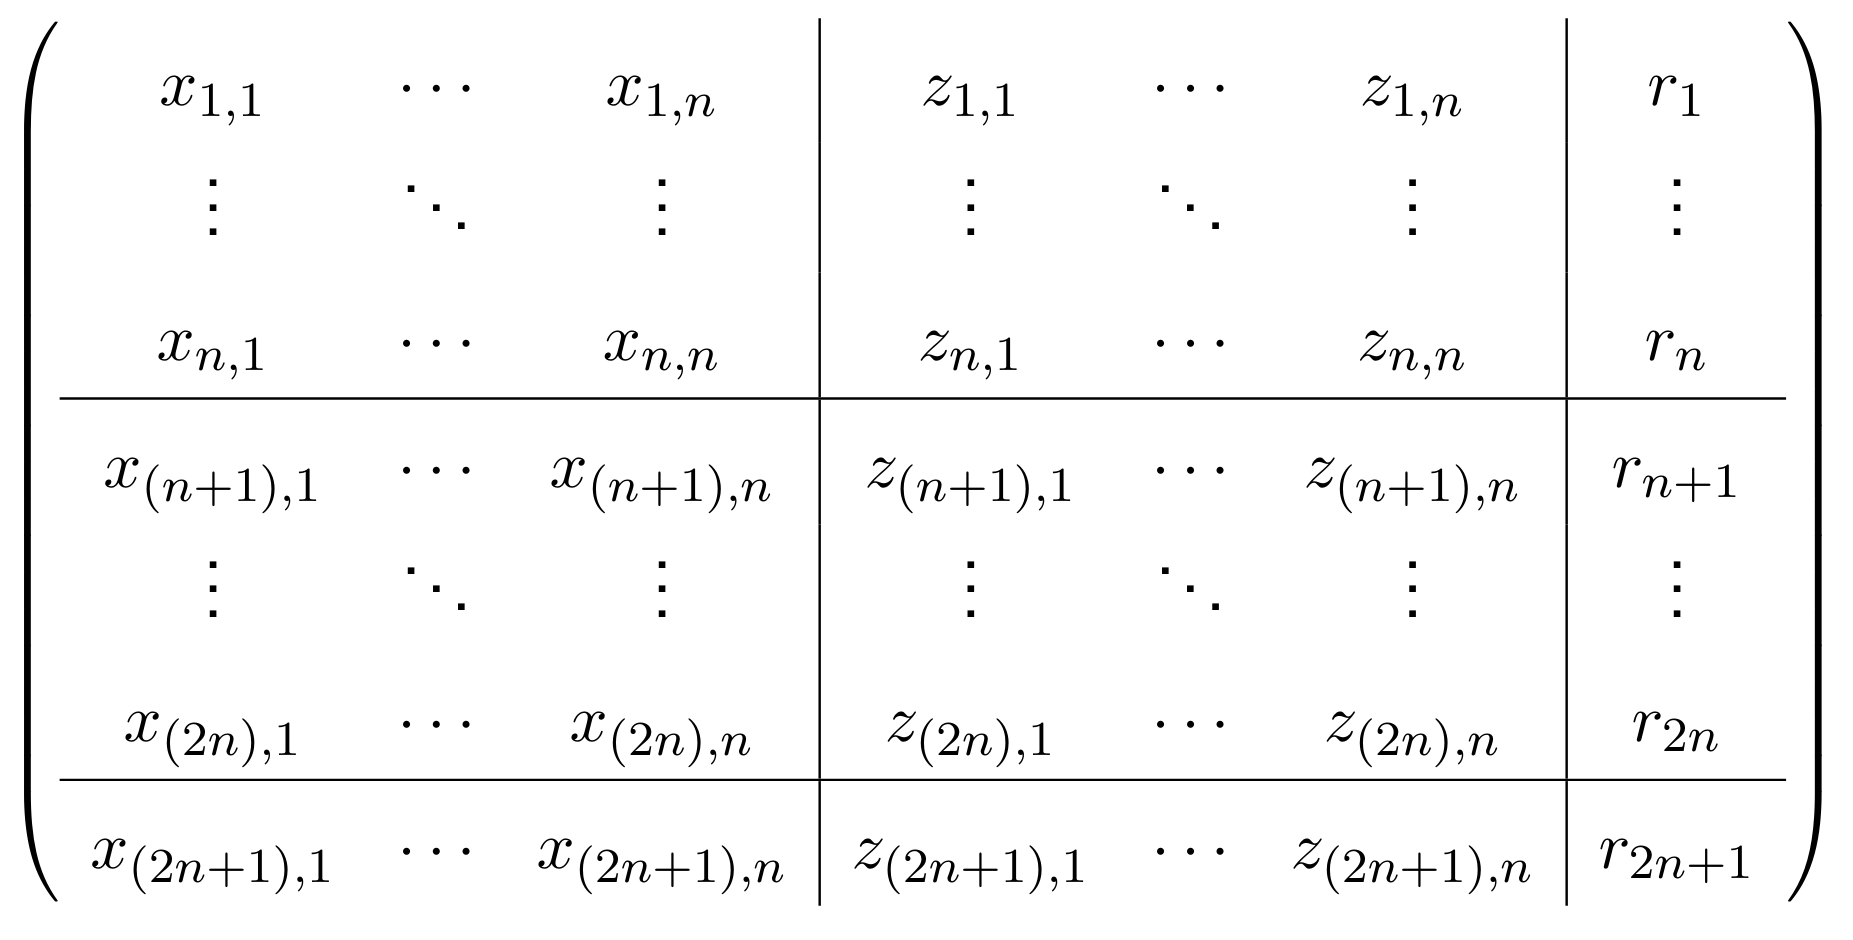
\includegraphics[scale=0.15]{images/CliffordTableau}
                \label{fig:clifford-tableau}
            \end{figure}
        }
    \end{minipage}

    \vspace*{5mm}

    \fullfootcite{02_ImprovedSimulationOfStabilizerCircuits}
\end{frame}


\begin{frame}{Clifford Tableau}{Initial Tableau}
    Pauli-\(Z\) gates stabilize \(\ket{0}\) states and Pauli-\(X\) gates destabilize \(\ket{0}\) states.

    \onslide<2->{
        \vspace*{2mm}
        \(\qquad\Longrightarrow\)
        Tableau for \(\ket{0}^{\otimes n}\) has an Identity submatrix for its first \((2n)\times(2n)\) submatrix.
    }
    \onslide<3->{
        \[
            \text{Tableau for }\ket{00}\text{ is }
            \left(
            \begin{array}{cc|cc|c}
                1 & 0 & 0 & 0 & 0 \\
                0 & 1 & 0 & 0 & 0 \\
                \hline
                0 & 0 & 1 & 0 & 0 \\
                0 & 0 & 0 & 1 & 0 \\
                \hline
                0 & 0 & 0 & 0 & 0 \\
            \end{array}
            \right)
        \]
    }
    \onslide<4->{
        In the following slides, let \(R_i\) denote the \(i\)-th row of the stabilizer tableau.
    }

    \vspace*{10mm}

    \fullfootcite{02_ImprovedSimulationOfStabilizerCircuits}
\end{frame}







    \begin{frame}{References}
        \printbibliography
    \end{frame}

\end{document}
